% !TEX root =  ../master.tex

\chapter{Prozesse}
Im folgenden werden die durch unsere Anwendung implementieren Prozesse grob als ereignisgesteuerte Prozesskette (EPK) aufgezeigt. Dabei wurden die folgenden Hauptfunktionen identifiziert:
\begin{enumerate}
	\item Login
	\item Auswahl des Farbschematas
	\item Auswahl der Sprache
	\item Suche
	\item Klausuren und Prüfungen
	\item Kursverwaltung
	\item Kursfunktionen
	\item Aufgaben
\end{enumerate}

\section{Login}
	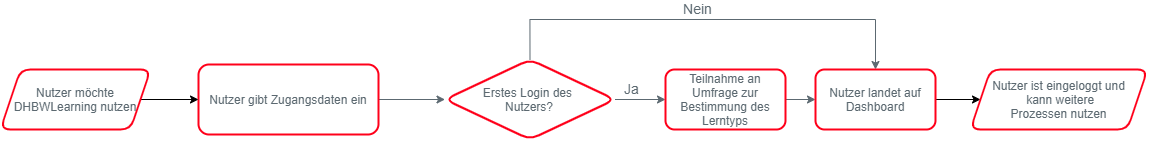
\includegraphics[width=\linewidth, keepaspectratio]{img/Prozesse/login}
\section{Auswahl des Farbschematas}
	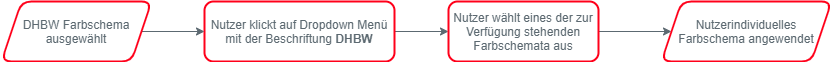
\includegraphics[width=\linewidth, keepaspectratio]{img/Prozesse/color}
\section{Auswahl der Sprache}
	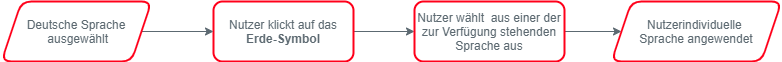
\includegraphics[width=\linewidth, keepaspectratio]{img/Prozesse/language}
\section{Suche}
	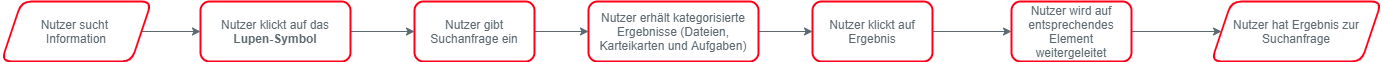
\includegraphics[width=\linewidth, keepaspectratio]{img/Prozesse/search}
\section{Klausuren und Prüfungen}
	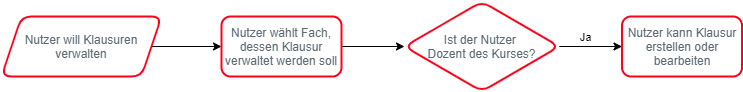
\includegraphics[width=\linewidth, keepaspectratio]{img/Prozesse/exams}

	\begin{landscape}
		\section{Kursverwaltung}
			\begin{figure}[!h]
				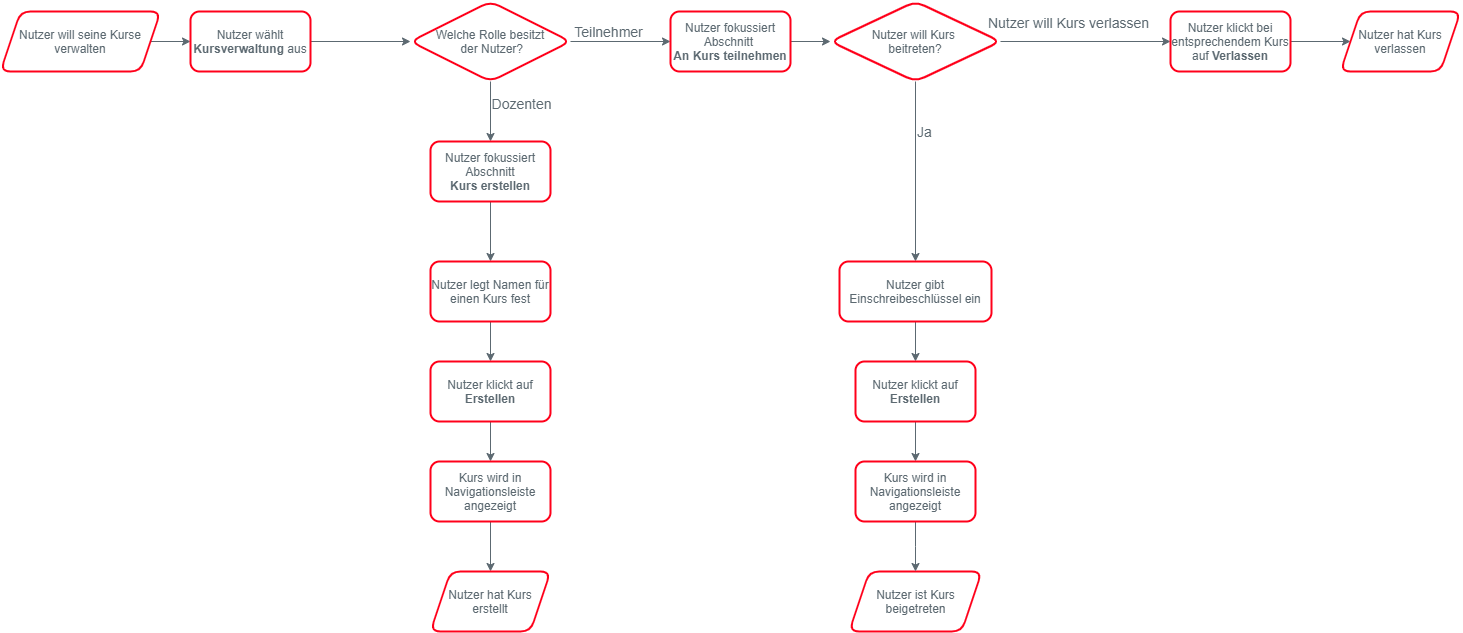
\includegraphics[width=\linewidth, keepaspectratio]{img/Prozesse/coursemanagement}
			\end{figure}
	\end{landscape}

	\begin{landscape}
		\section{Kursfunktionen}
			\begin{figure}[!h]
				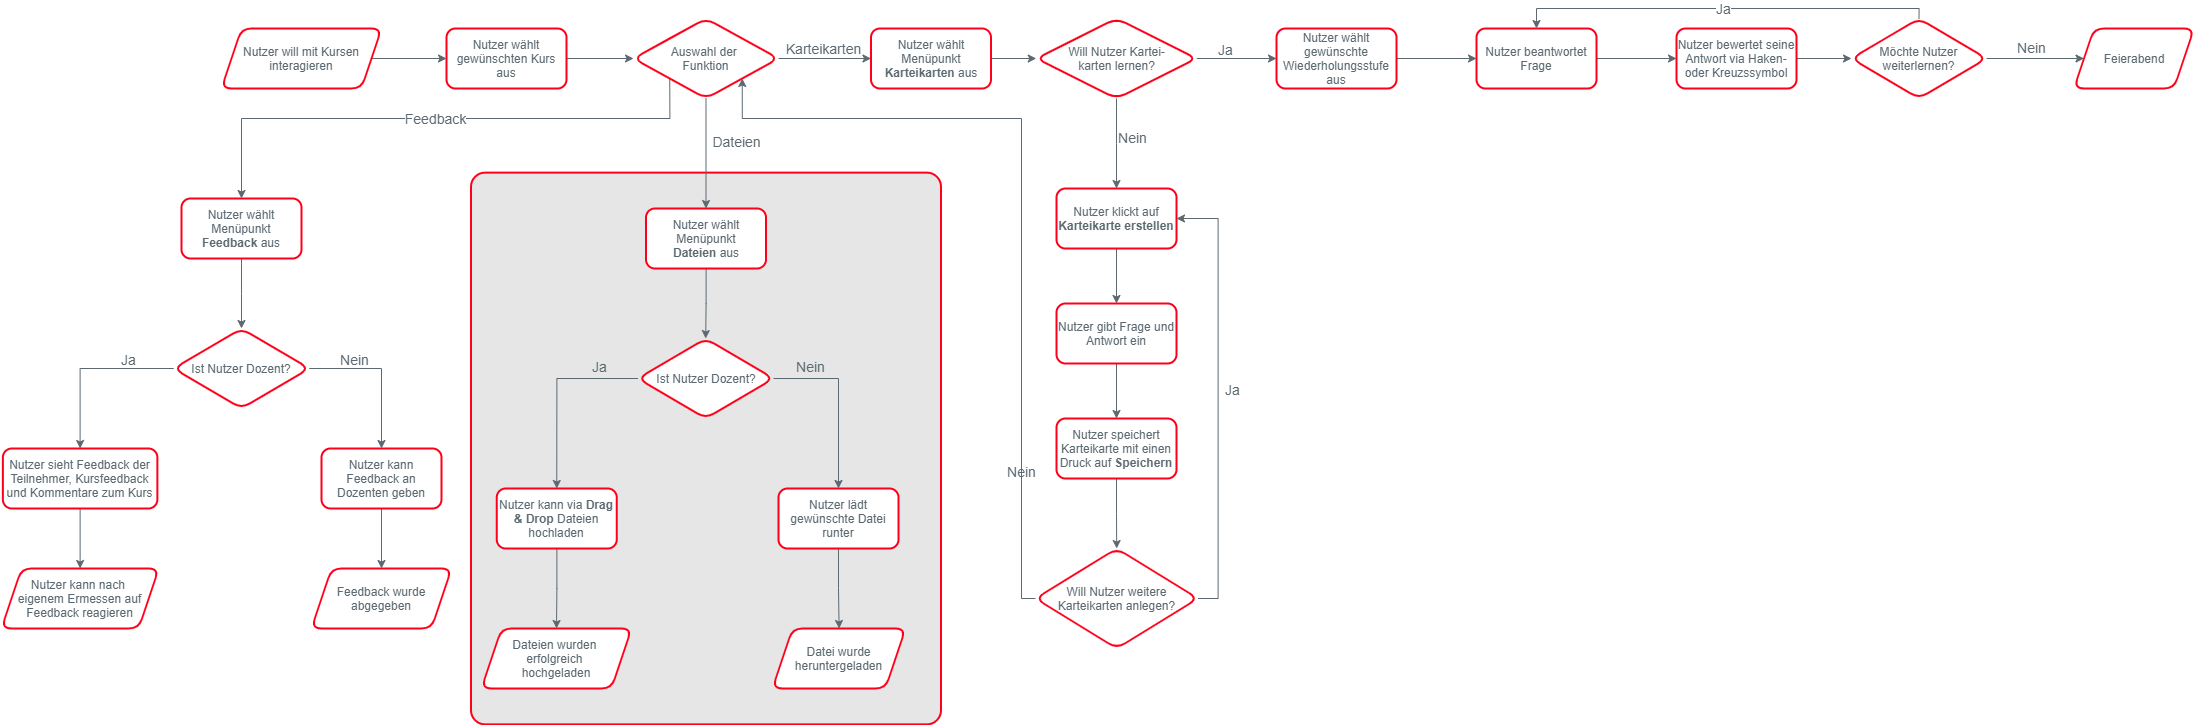
\includegraphics[width=\linewidth, keepaspectratio]{img/Prozesse/coursefunction}
			\end{figure}
	\end{landscape}

	\begin{landscape}
		\section{Aufgaben}
			\begin{figure}[!h]
				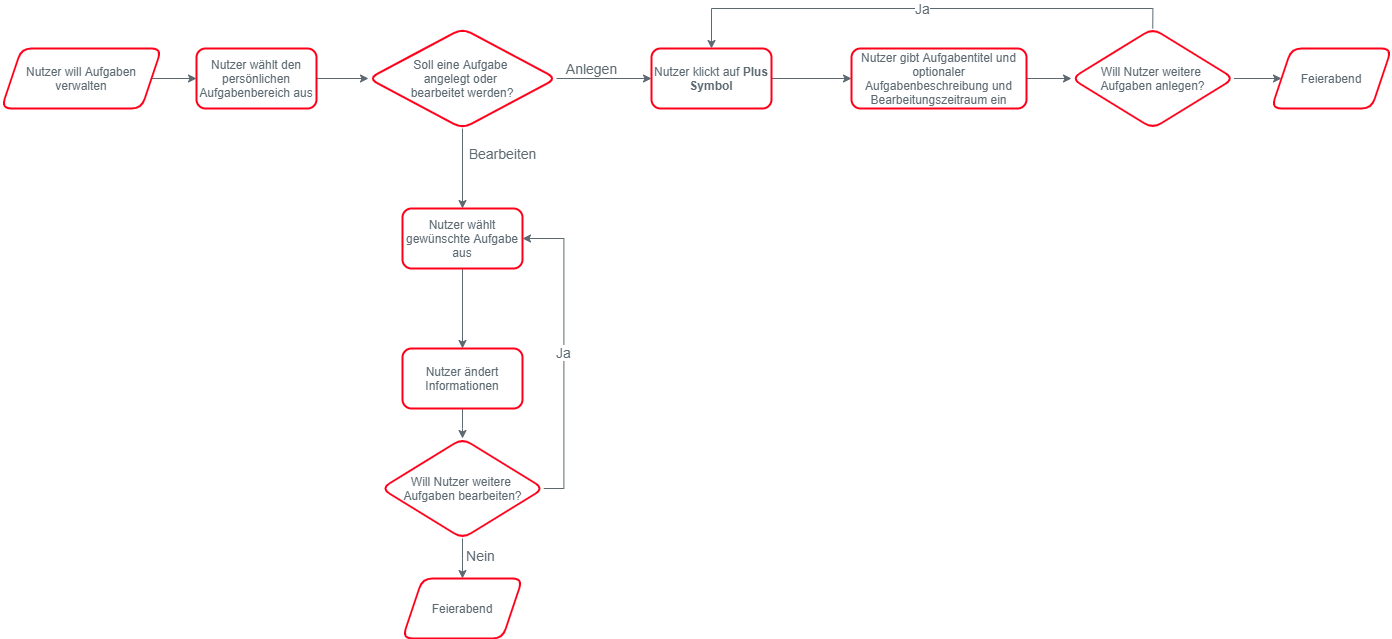
\includegraphics[width=\linewidth, keepaspectratio]{img/Prozesse/tasks}
			\end{figure}
	\end{landscape}
